\documentclass[review, authoryear]{elsarticle}\usepackage{graphicx, color}
%% maxwidth is the original width if it is less than linewidth
%% otherwise use linewidth (to make sure the graphics do not exceed the margin)
\makeatletter
\def\maxwidth{ %
  \ifdim\Gin@nat@width>\linewidth
    \linewidth
  \else
    \Gin@nat@width
  \fi
}
\makeatother

\IfFileExists{upquote.sty}{\usepackage{upquote}}{}
\definecolor{fgcolor}{rgb}{0.2, 0.2, 0.2}
\newcommand{\hlnumber}[1]{\textcolor[rgb]{0,0,0}{#1}}%
\newcommand{\hlfunctioncall}[1]{\textcolor[rgb]{0.501960784313725,0,0.329411764705882}{\textbf{#1}}}%
\newcommand{\hlstring}[1]{\textcolor[rgb]{0.6,0.6,1}{#1}}%
\newcommand{\hlkeyword}[1]{\textcolor[rgb]{0,0,0}{\textbf{#1}}}%
\newcommand{\hlargument}[1]{\textcolor[rgb]{0.690196078431373,0.250980392156863,0.0196078431372549}{#1}}%
\newcommand{\hlcomment}[1]{\textcolor[rgb]{0.180392156862745,0.6,0.341176470588235}{#1}}%
\newcommand{\hlroxygencomment}[1]{\textcolor[rgb]{0.43921568627451,0.47843137254902,0.701960784313725}{#1}}%
\newcommand{\hlformalargs}[1]{\textcolor[rgb]{0.690196078431373,0.250980392156863,0.0196078431372549}{#1}}%
\newcommand{\hleqformalargs}[1]{\textcolor[rgb]{0.690196078431373,0.250980392156863,0.0196078431372549}{#1}}%
\newcommand{\hlassignement}[1]{\textcolor[rgb]{0,0,0}{\textbf{#1}}}%
\newcommand{\hlpackage}[1]{\textcolor[rgb]{0.588235294117647,0.709803921568627,0.145098039215686}{#1}}%
\newcommand{\hlslot}[1]{\textit{#1}}%
\newcommand{\hlsymbol}[1]{\textcolor[rgb]{0,0,0}{#1}}%
\newcommand{\hlprompt}[1]{\textcolor[rgb]{0.2,0.2,0.2}{#1}}%

\usepackage{framed}
\makeatletter
\newenvironment{kframe}{%
 \def\at@end@of@kframe{}%
 \ifinner\ifhmode%
  \def\at@end@of@kframe{\end{minipage}}%
  \begin{minipage}{\columnwidth}%
 \fi\fi%
 \def\FrameCommand##1{\hskip\@totalleftmargin \hskip-\fboxsep
 \colorbox{shadecolor}{##1}\hskip-\fboxsep
     % There is no \\@totalrightmargin, so:
     \hskip-\linewidth \hskip-\@totalleftmargin \hskip\columnwidth}%
 \MakeFramed {\advance\hsize-\width
   \@totalleftmargin\z@ \linewidth\hsize
   \@setminipage}}%
 {\par\unskip\endMakeFramed%
 \at@end@of@kframe}
\makeatother

\definecolor{shadecolor}{rgb}{.97, .97, .97}
\definecolor{messagecolor}{rgb}{0, 0, 0}
\definecolor{warningcolor}{rgb}{1, 0, 1}
\definecolor{errorcolor}{rgb}{1, 0, 0}
\newenvironment{knitrout}{}{} % an empty environment to be redefined in TeX

\usepackage{alltt}
\usepackage{fullpage}

% remove Elsevier preprint footer
\makeatletter
\def\ps@pprintTitle{%
 \let\@oddhead\@empty
 \let\@evenhead\@empty
 \def\@oddfoot{}%
 \let\@evenfoot\@oddfoot}
\makeatother

%hyperrefs
\usepackage{hyperref}

% Math
\usepackage{amsmath}

% Color (for drafts)
\usepackage{color}
\usepackage[usenames, dvipsnames]{xcolor}



%==============================================================================
\begin{document}
\begin{knitrout}
\definecolor{shadecolor}{rgb}{0.969, 0.969, 0.969}\color{fgcolor}\begin{kframe}


{\ttfamily\noindent\itshape\textcolor{messagecolor}{\#\# Loading required package: Defaults}}

{\ttfamily\noindent\itshape\textcolor{messagecolor}{\#\# Loading required package: xts}}

{\ttfamily\noindent\itshape\textcolor{messagecolor}{\#\# Loading required package: zoo}}

{\ttfamily\noindent\itshape\textcolor{messagecolor}{\#\# \\\#\# Attaching package: 'zoo'\\\#\# }}

{\ttfamily\noindent\itshape\textcolor{messagecolor}{\#\# The following object(s) are masked from 'package:base':\\\#\# \\\#\#     as.Date, as.Date.numeric\\\#\# }}

{\ttfamily\noindent\itshape\textcolor{messagecolor}{\#\# Loading required package: TTR}}\end{kframe}
\end{knitrout}

%==============================================================================
\begin{frontmatter}
\title{Estimating Traffic Volumes in Athens: TRB data analysis competition}

\author[gtcivil]{Bhargava R. Chilukuri}
  \ead{bchilukuri3@gatech.edu}
\author[gtcivil]{Adnan Sheikh}
  \ead{asheikh7@gatech.edu}
\author[gtcivil,gtecon]{Gregory S. Macfarlane\corref{cor1}} 
  \ead{gregmacfarlane@gatech.edu}

\address[gtcivil]{School of Civil and Environmental Engineering, Georgia Institute of
Technology\\ 790 Atlantic Drive, Atlanta GA 30332-0355}
\address[gtecon]{School of Economics, Georgia Institute of Technology\\ 221 Bobby
Dodd Way, Atlanta, GA 30332}

% make footnote text referenced above
\cortext[cor1]{Corresponding author. Tel.: +1 801 616 9822}

%% Abstract
\begin{abstract}
Traffic loop detectors are important tools for recording and monitoring vehicle
flows along major routes in a region. The reliability of these detectors, 
however, is such that certain important observations may be missing. In this 
study, we employ an approach based on traffic flow theory and joined with
time series econometrics to impute missing values, and make modest projections,
from loop detector data in Athens, Greece.
\end{abstract}

% keywords environment
\begin{keyword}% separate with \sep
TRB data analysis competition \sep traffic forecasting 
\end{keyword}
\end{frontmatter}
%==============================================================================

\section{Introduction}

%------------------------------------------------------------------------------
\subsection{Literature}


%==============================================================================
\section{Model}
\begin{knitrout}
\definecolor{shadecolor}{rgb}{0.969, 0.969, 0.969}\color{fgcolor}\begin{kframe}
\begin{alltt}
MyData <- \hlfunctioncall{read.csv}(\hlstring{"./Source_Data/data_additional_April.csv"})
lanes <- \hlfunctioncall{c}(1, 2, 3, 4, 6, 7, 8)


\hlcomment{# Convert timestamp}
MyData$TIMESTAMP <- \hlfunctioncall{as.POSIXct}(\hlfunctioncall{strptime}(MyData$TIMESTAMP, format = \hlstring{"%m/%d/%y %H:%M"}))

\hlcomment{# change 255 for missing}

\hlcomment{# critical occupancy dummy}
MyData$L101_crit <- \hlfunctioncall{ifelse}(MyData$L101_occupancy > 20, 1, 0)

\hlcomment{# throw away volume outliers}
MyData$L101_volume <- \hlfunctioncall{ifelse}(MyData$L101_volume > 100, NA, MyData$L101_volume)
\end{alltt}
\end{kframe}
\end{knitrout}

%------------------------------------------------------------------------------
\subsection{Estimation}
We estimate an autoregressive model for each lane, and present the coefficient estimates 
in Table \ref{tab:AR1Coefficients}

\begin{knitrout}
\definecolor{shadecolor}{rgb}{0.969, 0.969, 0.969}\color{fgcolor}\begin{kframe}
\begin{alltt}
model1lag <- \hlfunctioncall{lm}(L101_volume ~ \hlfunctioncall{Lag}(L101_volume, k = 1), data = MyData)
model1lagc <- \hlfunctioncall{lm}(L101_volume ~ \hlfunctioncall{Lag}(L101_volume, k = 1) + L101_crit, 
    data = MyData)
model1int <- \hlfunctioncall{lm}(L101_volume ~ \hlfunctioncall{Lag}(L101_volume, k = 1) + L101_crit + 
    \hlfunctioncall{Lag}(L101_volume, k = 1):L101_crit, data = MyData)
model2lag <- \hlfunctioncall{lm}(L101_volume ~ \hlfunctioncall{Lag}(L101_volume, k = 1):L101_crit + 
    \hlfunctioncall{Lag}(L101_volume, k = 1) + L101_crit + \hlfunctioncall{Lag}(L101_volume, k = 2), data = MyData)
\end{alltt}
\end{kframe}
\end{knitrout}


\begin{table}
  \caption{Loop1 models}
\begin{knitrout}
\definecolor{shadecolor}{rgb}{0.969, 0.969, 0.969}\color{fgcolor}\begin{kframe}
\begin{alltt}
\hlfunctioncall{apsrtable}(model1lag, model1lagc, model1int, model2lag, Sweave = TRUE, 
    coefrows = 1, digits = 4)
\end{alltt}


{\ttfamily\noindent\bfseries\textcolor{errorcolor}{\#\# Error: \$ operator is invalid for atomic vectors}}\end{kframe}
\end{knitrout}

\end{table}

\begin{knitrout}
\definecolor{shadecolor}{rgb}{0.969, 0.969, 0.969}\color{fgcolor}\begin{kframe}
\begin{alltt}
model1 <- \hlfunctioncall{lm}(L101_volume ~ \hlfunctioncall{Lag}(L101_volume, k = 1):L101_crit + \hlfunctioncall{Lag}(L101_volume, 
    k = 1) + L101_crit + \hlfunctioncall{Lag}(L101_volume, k = 960), data = MyData)
model2 <- \hlfunctioncall{lm}(L102_volume ~ \hlfunctioncall{Lag}(L102_volume, k = 1), data = MyData)
model3 <- \hlfunctioncall{lm}(L103_volume ~ \hlfunctioncall{Lag}(L103_volume, k = 1), data = MyData)
model4 <- \hlfunctioncall{lm}(L104_volume ~ \hlfunctioncall{Lag}(L104_volume, k = 1), data = MyData)
model6 <- \hlfunctioncall{lm}(L106_volume ~ \hlfunctioncall{Lag}(L106_volume, k = 1), data = MyData)
model7 <- \hlfunctioncall{lm}(L107_volume ~ \hlfunctioncall{Lag}(L107_volume, k = 1), data = MyData)
model8 <- \hlfunctioncall{lm}(L108_volume ~ \hlfunctioncall{Lag}(L108_volume, k = 1), data = MyData)
AR1models <- \hlfunctioncall{list}(model1, model2, model3, model4, model6, model7, 
    model8)
\end{alltt}
\end{kframe}
\end{knitrout}




\begin{table}
  \caption{Autoregressive Model Coefficients}
  \label{tab:AR1Coefficients}
  \begin{center}
\begin{kframe}
\begin{alltt}
AR1Coefs <- \hlfunctioncall{as.table}(\hlfunctioncall{matrix}(NA, ncol = \hlfunctioncall{length}(AR1models), nrow = 3))
\hlfunctioncall{for} (i in 1:\hlfunctioncall{length}(AR1models)) \{
    AR1Coefs[1:2, i] <- \hlfunctioncall{t}(\hlfunctioncall{coef}(AR1models[[i]]))
    AR1Coefs[3, i] <- \hlfunctioncall{summary}(AR1models[[i]])$r.squared
    \hlfunctioncall{colnames}(AR1Coefs)[i] <- \hlfunctioncall{paste}(\hlstring{"Lane "}, lanes[i], sep = \hlstring{""})
\}
\end{alltt}


{\ttfamily\noindent\bfseries\textcolor{errorcolor}{\#\# Error: number of items to replace is not a multiple of replacement length}}\begin{alltt}
\hlfunctioncall{rownames}(AR1Coefs) <- \hlfunctioncall{c}(\hlstring{"Intercept"}, \hlstring{"Lag"}, \hlstring{"$R^2$"})

coefs.x <- \hlfunctioncall{xtable}(AR1Coefs)
\hlfunctioncall{print}(coefs.x, floating = FALSE, sanitize.rownames.function = \hlfunctioncall{function}(x) \{
    x
\})
\end{alltt}
\end{kframe}
% latex table generated in R 2.15.0 by xtable 1.7-0 package
% Thu Nov 15 14:09:21 2012
\begin{tabular}{rlllllll}
  \hline
 & A & B & C & D & E & F & G \\ 
  \hline
Intercept &  &  &  &  &  &  &  \\ 
  Lag &  &  &  &  &  &  &  \\ 
  $R^2$ &  &  &  &  &  &  &  \\ 
   \hline
\end{tabular}



  \end{center}
\end{table}

\begin{knitrout}
\definecolor{shadecolor}{rgb}{0.969, 0.969, 0.969}\color{fgcolor}\begin{kframe}
\begin{alltt}
model21 <- \hlfunctioncall{lm}(L101_volume ~ \hlfunctioncall{Lag}(L101_volume, k = 1) + \hlfunctioncall{Lag}(L101_volume, 
    k = 2), data = MyData)
model22 <- \hlfunctioncall{lm}(L102_volume ~ \hlfunctioncall{Lag}(L102_volume, k = 1) + \hlfunctioncall{Lag}(L102_volume, 
    k = 2), data = MyData)
model23 <- \hlfunctioncall{lm}(L103_volume ~ \hlfunctioncall{Lag}(L103_volume, k = 1) + \hlfunctioncall{Lag}(L103_volume, 
    k = 2), data = MyData)
model24 <- \hlfunctioncall{lm}(L104_volume ~ \hlfunctioncall{Lag}(L104_volume, k = 1) + \hlfunctioncall{Lag}(L104_volume, 
    k = 2), data = MyData)
model26 <- \hlfunctioncall{lm}(L106_volume ~ \hlfunctioncall{Lag}(L106_volume, k = 1) + \hlfunctioncall{Lag}(L106_volume, 
    k = 2), data = MyData)
model27 <- \hlfunctioncall{lm}(L107_volume ~ \hlfunctioncall{Lag}(L107_volume, k = 1) + \hlfunctioncall{Lag}(L107_volume, 
    k = 2), data = MyData)
model28 <- \hlfunctioncall{lm}(L108_volume ~ \hlfunctioncall{Lag}(L108_volume, k = 1) + \hlfunctioncall{Lag}(L108_volume, 
    k = 2), data = MyData)
AR2models <- \hlfunctioncall{list}(model21, model22, model23, model24, model26, model27, 
    model28)
\end{alltt}
\end{kframe}
\end{knitrout}




\begin{table}
  \caption{Autoregressive  2 Model Coefficients}
  \label{tab:AR2Coefficients}
  \begin{center}
\begin{kframe}
\begin{alltt}
AR2Coefs <- \hlfunctioncall{as.table}(\hlfunctioncall{matrix}(NA, ncol = \hlfunctioncall{length}(AR1models), nrow = 4))
\hlfunctioncall{for} (i in 1:\hlfunctioncall{length}(AR1models)) \{
    AR2Coefs[1:3, i] <- \hlfunctioncall{t}(\hlfunctioncall{coef}(AR2models[[i]]))
    AR2Coefs[4, i] <- \hlfunctioncall{summary}(AR2models[[i]])$r.squared
    \hlfunctioncall{colnames}(AR1Coefs)[i] <- \hlfunctioncall{paste}(\hlstring{"Lane "}, lanes[i], sep = \hlstring{""})
\}
\hlfunctioncall{rownames}(AR2Coefs) <- \hlfunctioncall{c}(\hlstring{"Intercept"}, \hlstring{"Lag"}, \hlstring{"Lag-2"}, \hlstring{"$R^2$"})

coefs.x <- \hlfunctioncall{xtable}(AR2Coefs)
\hlfunctioncall{print}(coefs.x, floating = FALSE, sanitize.rownames.function = \hlfunctioncall{function}(x) \{
    x
\})
\end{alltt}
\end{kframe}
% latex table generated in R 2.15.0 by xtable 1.7-0 package
% Thu Nov 15 14:09:26 2012
\begin{tabular}{rrrrrrrr}
  \hline
 & A & B & C & D & E & F & G \\ 
  \hline
Intercept & 4.65 & 3.55 & 3.88 & 7.71 & 8.12 & 3.18 & 3.53 \\ 
  Lag & 0.44 & 0.47 & 0.57 & 0.57 & 0.49 & 0.49 & 0.59 \\ 
  Lag-2 & 0.42 & 0.44 & 0.33 & 0.19 & 0.33 & 0.41 & 0.30 \\ 
  $R^2$ & 0.67 & 0.76 & 0.75 & 0.50 & 0.60 & 0.76 & 0.75 \\ 
   \hline
\end{tabular}



  \end{center}
\end{table}

\begin{knitrout}
\definecolor{shadecolor}{rgb}{0.969, 0.969, 0.969}\color{fgcolor}\begin{kframe}
\begin{alltt}
\hlfunctioncall{plot}(MyData$L101_occupancy[3 * (1:960)], MyData$L101_volume[3 * (1:960)], 
    main = \hlstring{"Day 3, Loop 1"})
\end{alltt}
\end{kframe}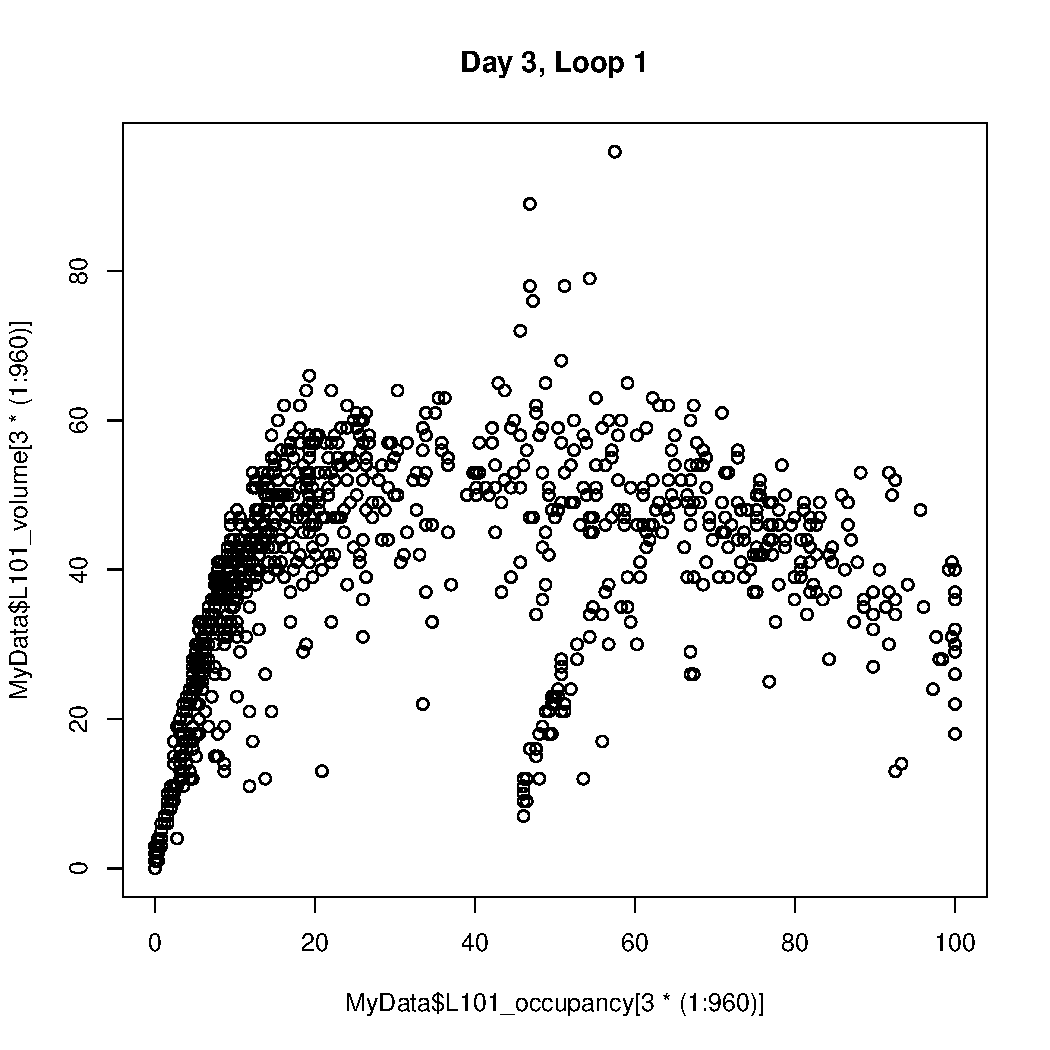
\includegraphics[width=\maxwidth]{figure/unnamed-chunk-11} \begin{kframe}\begin{alltt}
\hlfunctioncall{plot}(MyData$L102_occupancy[3 * (1:960)], MyData$L102_volume[3 * (1:960)], 
    main = \hlstring{"Day 3, Loop 2"}, ylim = \hlfunctioncall{c}(0, 100))
\end{alltt}
\end{kframe}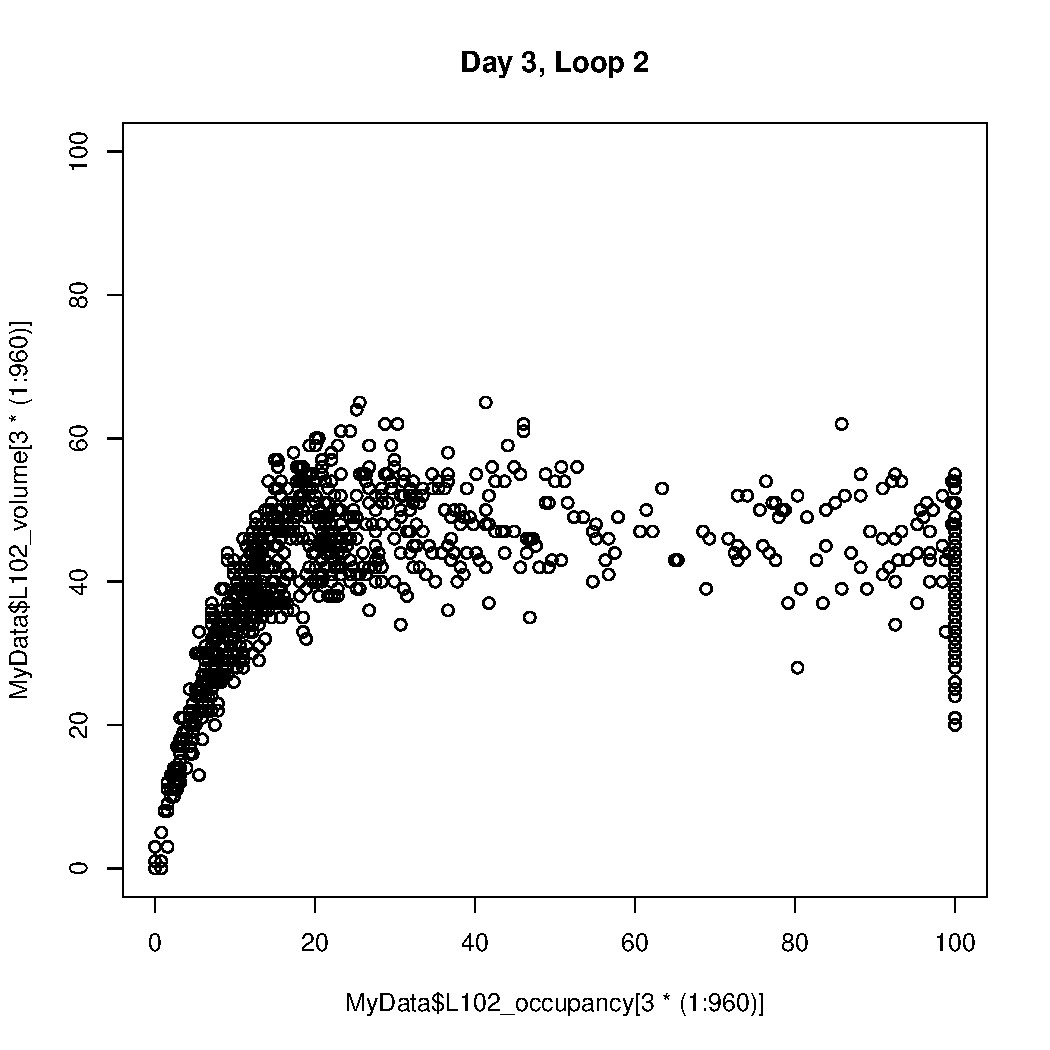
\includegraphics[width=\maxwidth]{figure/unnamed-chunk-12} \begin{kframe}\begin{alltt}
\hlfunctioncall{plot}(MyData$L103_occupancy[3 * (1:960)], MyData$L103_volume[3 * (1:960)], 
    main = \hlstring{"Day 3, Loop 3"}, ylim = \hlfunctioncall{c}(0, 100))
\end{alltt}
\end{kframe}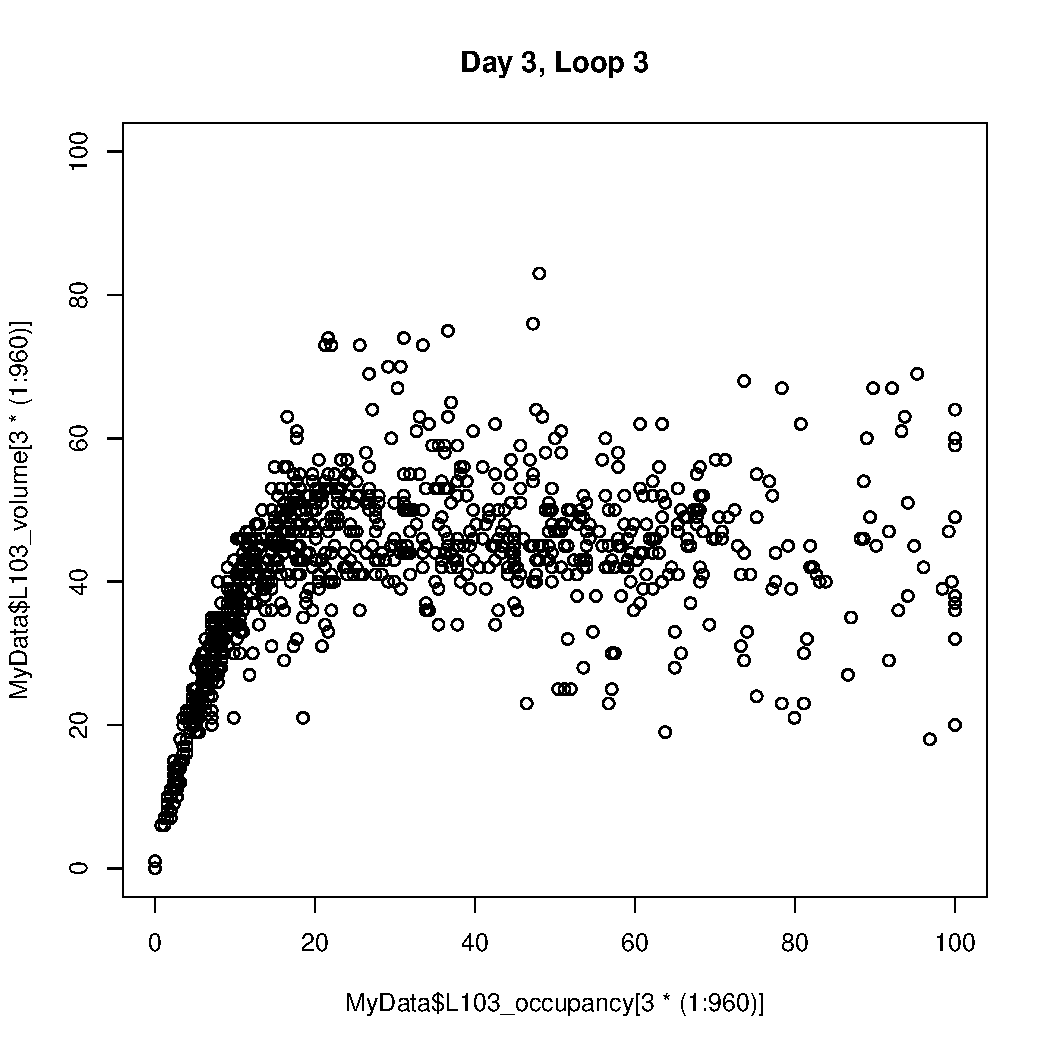
\includegraphics[width=\maxwidth]{figure/unnamed-chunk-13} \begin{kframe}\begin{alltt}
\hlfunctioncall{plot}(MyData$L104_occupancy[10 * (1:960)], MyData$L104_volume[10 * 
    (1:960)], main = \hlstring{"Day 3, Loop 4"}, ylim = \hlfunctioncall{c}(0, 100))
\end{alltt}
\end{kframe}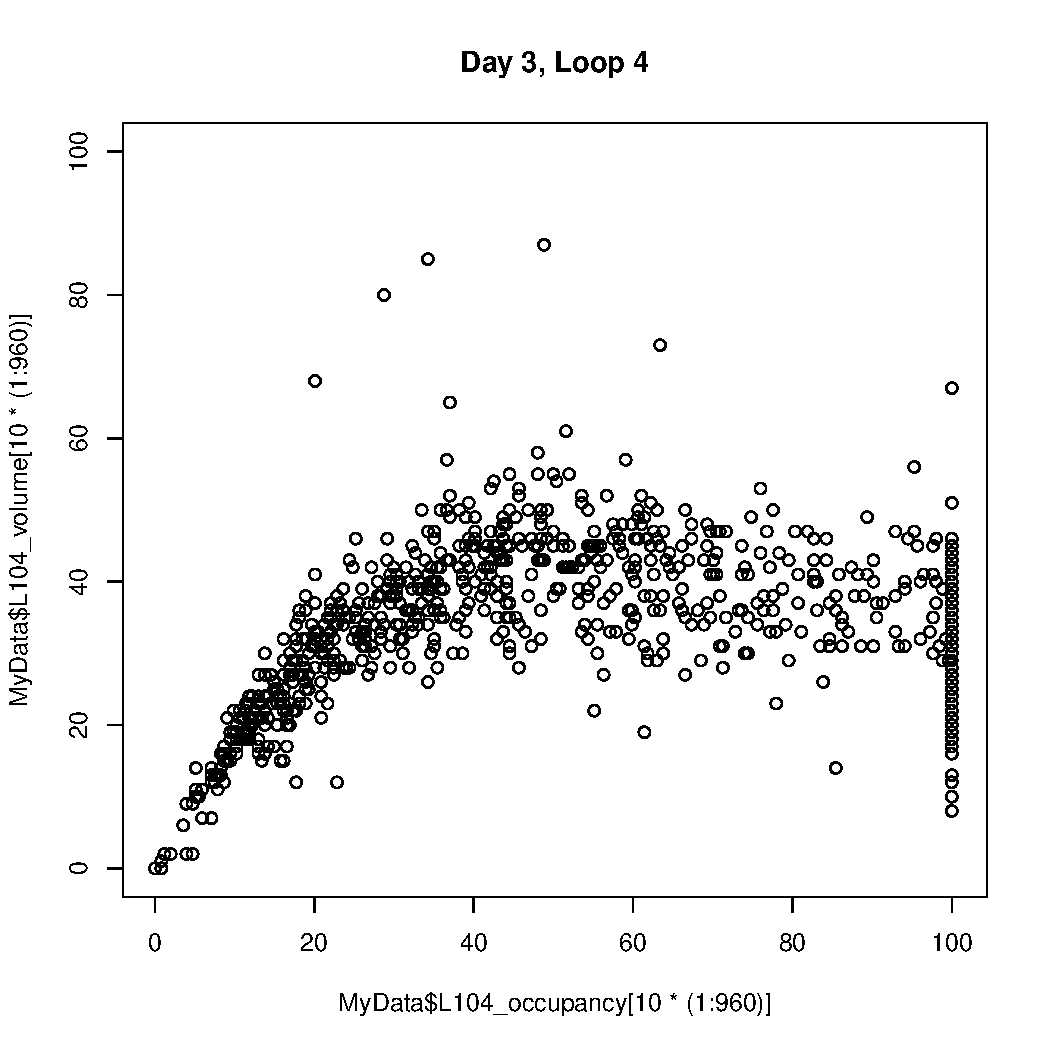
\includegraphics[width=\maxwidth]{figure/unnamed-chunk-14} \begin{kframe}\begin{alltt}
\hlfunctioncall{plot}(MyData$L106_occupancy[3 * (1:960)], MyData$L106_volume[3 * (1:960)], 
    main = \hlstring{"Day 3, Loop 6"}, ylim = \hlfunctioncall{c}(0, 100))
\end{alltt}
\end{kframe}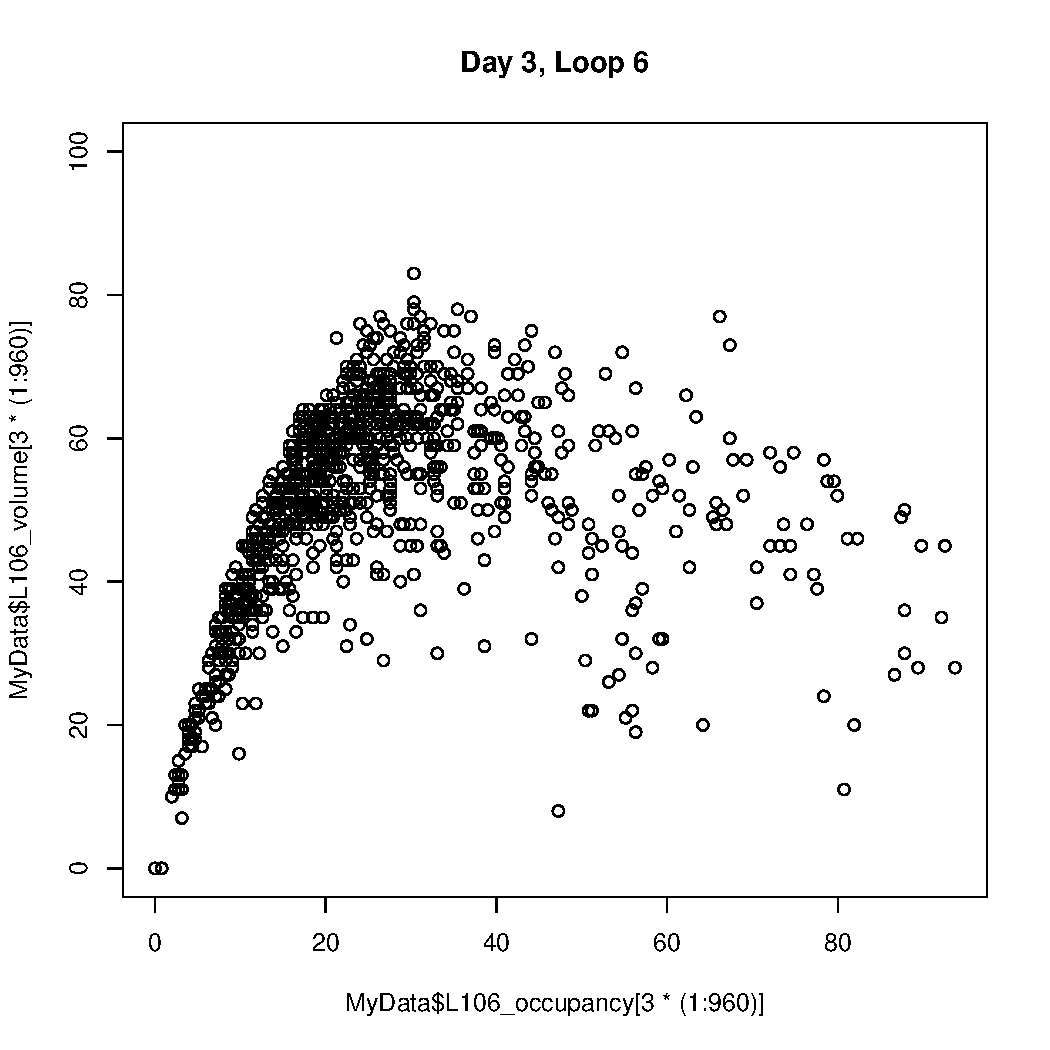
\includegraphics[width=\maxwidth]{figure/unnamed-chunk-15} \begin{kframe}\begin{alltt}
\hlfunctioncall{plot}(MyData$L107_occupancy[3 * (1:960)], MyData$L107_volume[3 * (1:960)], 
    main = \hlstring{"Day 3, Loop 7"}, ylim = \hlfunctioncall{c}(0, 100))
\end{alltt}
\end{kframe}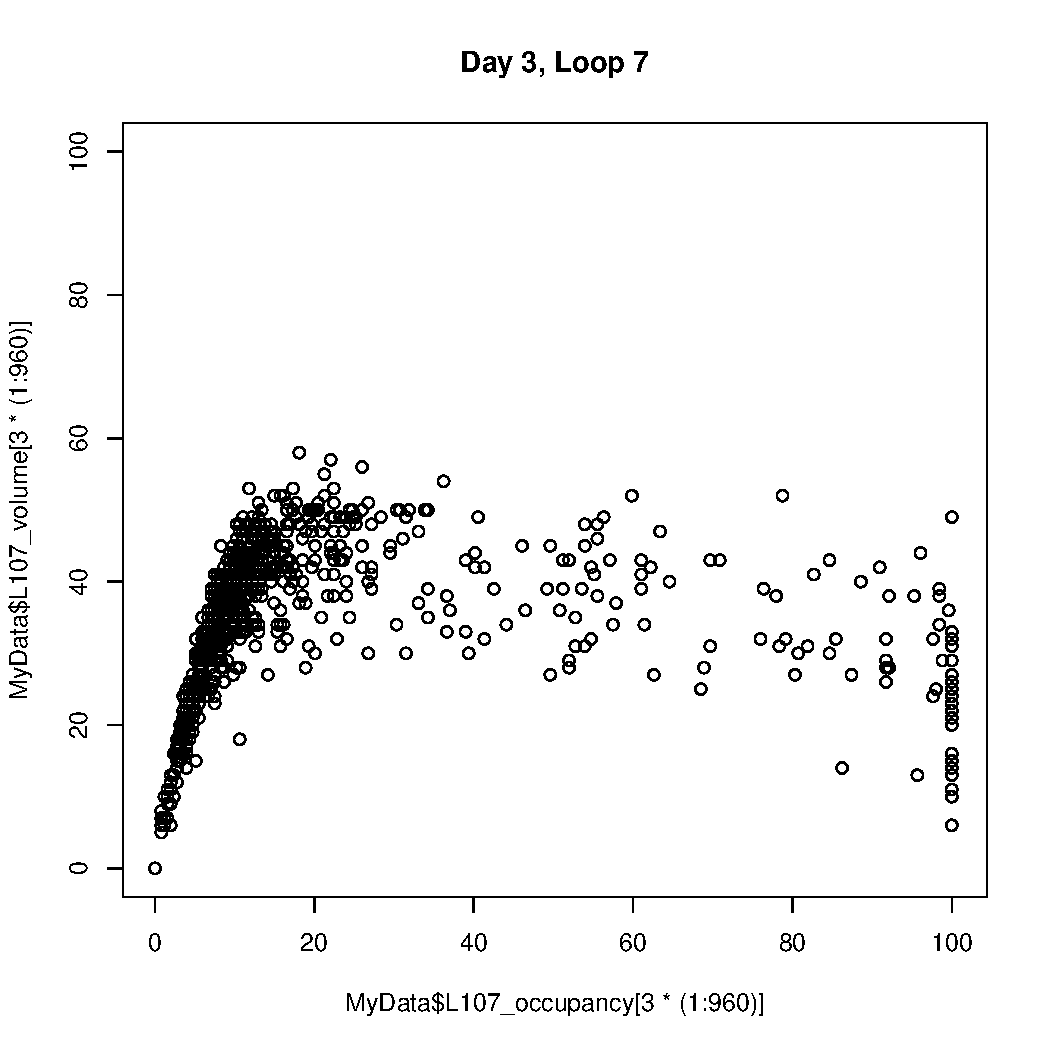
\includegraphics[width=\maxwidth]{figure/unnamed-chunk-16} \begin{kframe}\begin{alltt}
\hlfunctioncall{plot}(MyData$L108_occupancy[3 * (1:960)], MyData$L108_volume[3 * (1:960)], 
    main = \hlstring{"Day 3, Loop 8"}, ylim = \hlfunctioncall{c}(0, 100))
\end{alltt}
\end{kframe}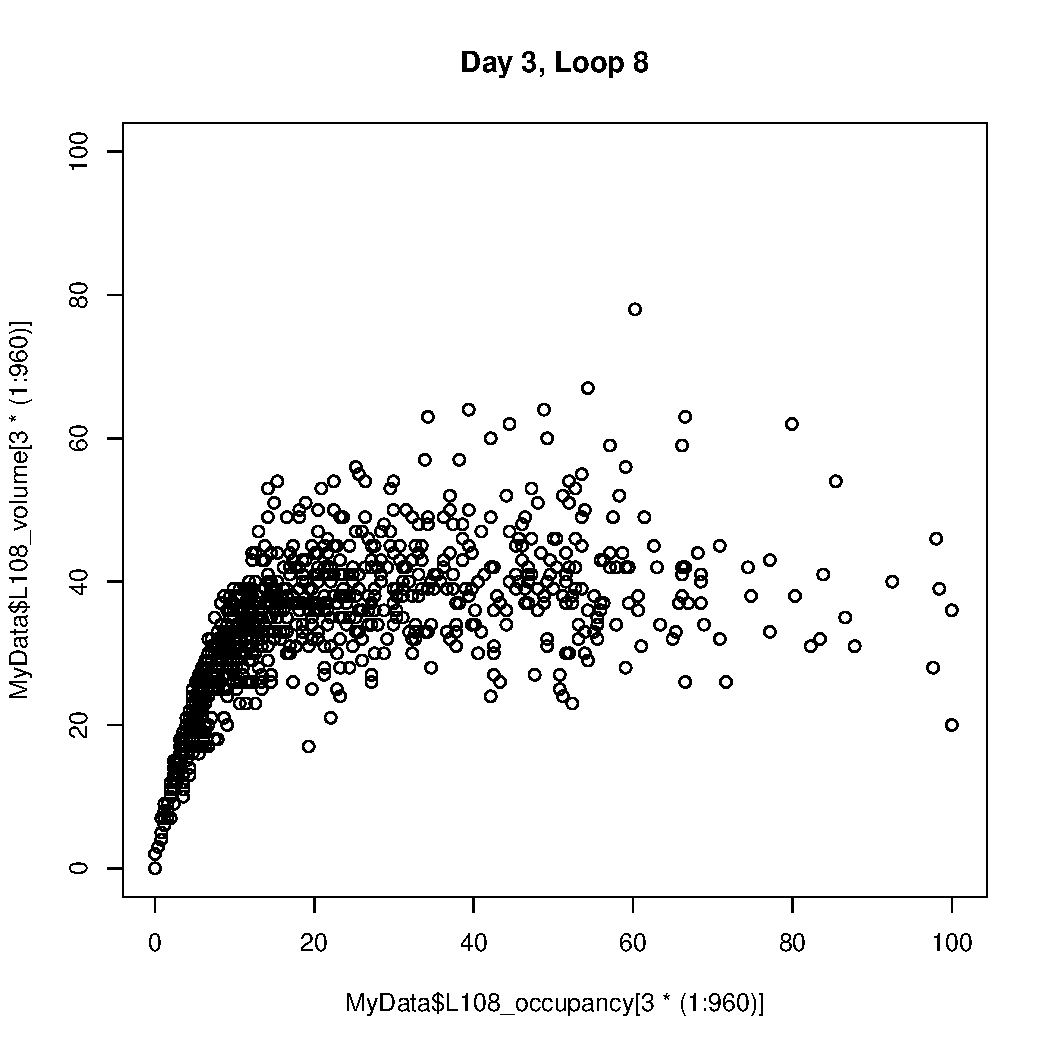
\includegraphics[width=\maxwidth]{figure/unnamed-chunk-17} 
\end{knitrout}



%==============================================================================
\section{Forecasting}


%==============================================================================
\section{Conclusion}

\subsection*{A word on execution}
This project was executed as a training exercise on literate programming using 
R \citep{R}, \texttt{knitr} \citep{knitr}, and \LaTeX. The source code is available
on GitHub as the 
\href{https://github.com/gregmacfarlane/GT_TranspoComp}{\texttt{GT\_TranspoComp}}
project.


\section*{References}
\bibliographystyle{elsarticle-num-names}
\bibliography{bibliography}
\end{document}
